\documentclass[12pt]{article}
\usepackage[utf8]{inputenc}
\usepackage[T2A]{fontenc}
\usepackage[russian]{babel}
\usepackage{amsmath}
\usepackage{amssymb}
\usepackage{dsfont}
\usepackage[dvipsnames]{xcolor}
\usepackage{setspace}
\usepackage{multirow}
\usepackage[a4paper, outer=1.5cm, inner=1.5cm, top=1cm, bottom=1cm]{geometry}
\usepackage{graphicx}
\usepackage{skull}
\usepackage{wasysym}
\usepackage{float}
\graphicspath{{.images/}}
\usepackage{hyperref}
\hypersetup{colorlinks=true, linkcolor=blue, filecolor=magenta, urlcolor=cyan}
\usepackage[firstpage]{draftwatermark}
\SetWatermarkText{
    $\qquad\qquad\qquad\qquad\qquad$\parbox{7cm}{\begin{center}
    
\includegraphics[width = 0.08\textwidth]{lion-logo.png}\bigskip\\~\bigskip\\~\vspace{-24mm}\\~\end{center}}
}
\SetWatermarkAngle{0}
\SetWatermarkScale{1.5}
\usepackage{etoolbox}

\newtoggle{ifsolved}
\newtoggle{needhelp}
\newcounter{num}
\setcounter{num}{1}

\newcommand{\newnum}{\par\textbf{\textnumero\arabic{num}}\stepcounter{num}}
\newcommand{\sol}{\vspace{3mm}\par\textbf{Решение: }}
\newcommand{\ans}{\vspace{3mm}\par\textbf{Ответ: }}
\newcommand{\hint}{\vspace{3mm}\par\textbf{Подсказка: }}
\newcommand{\mode}[1]{
\ifstrequal{#1}{0}{\togglefalse{ifsolved}\togglefalse{needhelp}}{\ifstrequal{#1}{1}{\togglefalse{ifsolved}\toggletrue{needhelp}}{\ifstrequal{#1}{2}{\toggletrue{ifsolved}\togglefalse{needhelp}}{\toggletrue{ifsolved}\toggletrue{needhelp}}}}} %if 0 - if 1 - if 2 - else
%\newenvironment{problem}[8]{%#1, #2, #3
%\parbox{\linewidth}{\vspace{4mm}\ifstrequal{#4}{(лёгкая)}{\newnum\textbf{.}}{\newnum\textbf{*.} } \\ #5}
%\iftoggle{ifsolved}{\sol #6}{}
%\iftoggle{ifsolved}{\ans #7}{}
%\iftoggle{needhelp}{\hint #8}{}}

\newenvironment{problem}[8]{%#1, #2, #3
\parbox{\linewidth}{\vspace{5mm}\ifstrequal{#4}{(лёгкая)}{\newnum\textbf{.}}{\newnum\textbf{*.} } \\ #5}
\iftoggle{ifsolved}{\sol #6}{}

\iftoggle{ifsolved}{\parbox{\linewidth}{\ans #7}}{}
\iftoggle{needhelp}{\parbox{\linewidth}{\hint #8}}{}}

\newenvironment{mylist} %custom list
{ \begin{itemize}
    \setlength{\itemsep}{0pt}
    \setlength{\parskip}{0pt}
    \setlength{\parsep}{0pt}     }
{ \end{itemize}                  }

\newenvironment{homeass}[1]{\vspace*{-1.5cm}
\iftoggle{ifsolved}{
    \section*{\center{Решение домашнего задания к #1.}}
}{
    \section*{\center{\textcolor{Sepia}{Домашнее задание к #1}}}
} \vspace{7mm}\large}

\parindent=0pt
\pagestyle{empty}
%$\!$[\arabic{class}.\arabic{num}]
%\ifnumcomp{\value{counter}}{>}{1}{true}{false}
%\definecolor{Gray}{gray}{0.9}
%\definecolor{mypink}{RGB}{219, 48, 122}
%\newcolumntype{g}{>{\columncolor{Gray}}p{2.8cm}}

\begin{document}
\large
\mode{7}
%0 for problems without hints
%1 for problems + hints
%2 for problems + solutions + answers
%else: show all

{\centering\section*{СПИСОК ЗАДАЧ}}

{\centering\subsection*{\smallskip\\\textcolor{green}{\textbf{Полезные вещи, которые можно и нужно копипастить:}}}}

\subsection*{\textcolor{Emerald}{\textbf{Полезные шпаргалки по LaTeXу:}}}

\textbf{Пример вставки рисунка:}

\begin{minipage}{\linewidth}
    \begin{minipage}{0.54\linewidth}
    см. рисунок справа\\
    Текст к собственно пикче, примерно всегда это либо развёрнутое описание, либо большая часть решения задачи --- стремимся экономить пространство, если это можно сделать.
    \end{minipage}
    \hspace{0.05\linewidth}
    \begin{minipage}{0.4\linewidth}
    \begin{figure}[H] 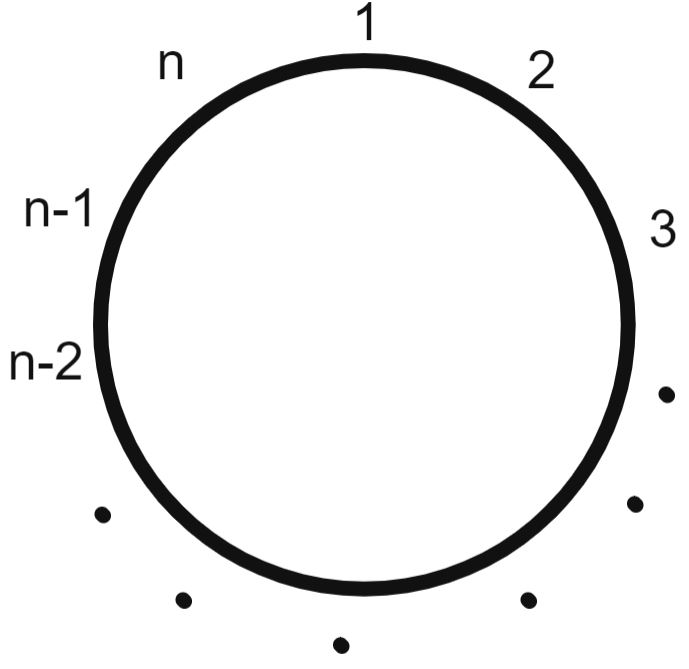
\includegraphics[width=\linewidth]{sol3} %тут поменять имя пикчи
    \end{figure}
    \end{minipage}
\end{minipage}

\textbf{Дефолтные математические знаки и символы:}\\
$\geqslant$,
$\leqslant$,
$a^{b}$,
$x_{i}$,
$\sqrt{a}$,
$\frac{a}{b}$,
$\displaystyle \frac{a}{b}$,
$\cdot$
$\;\Rightarrow\;$,
$\;\Leftrightarrow\;$,
$1{,}2$.
О промежутках:
$a\!b$,
$a\,b$,
$a\:b$,
$a\;b$,
$a\quad b$.

\textbf{Стандартные система и совокупность уравнений / неравенств:}\\
$\left\{
\begin{aligned}
f(x) &= 0 \\
g(x) &= 1
\end{aligned}\right.$

$\left[\begin{aligned}
&\left\{\begin{aligned}
f(x) &\geqslant a \\
g(x) &= b
\end{aligned}\right.\\
&\left\{\begin{aligned}
f(x) &< a \\
g(x) &= -b
\end{aligned}\right.
\end{aligned}\right.$

\subsection*{\textcolor{Emerald}{\textbf{Не математическое, но полезное:}}}
% комментарий в любом месте документа, который нигде не будет видно. Можно использовать для написания заметок-вопросов по задачам
\textbf{Пример таблицы:}

\begin{tabular}{|c|c|c|}
\hline
    $a$ & $b$ & текст
\\\hline
    $c$ & $d$ & мораль
\\\hline
\end{tabular}\\

\textbf{Отступы:} между\smallskip\\ строками\medskip\\ \textbf{Тире} --- это три дефиса.\\
\textbf{Списки:}
\begin{mylist}
\item [$\bullet$] это был пункт а
\item [2)] а это уже пункт номер 2 с изменённым заголовком
\end{mylist}

\subsection*{\textcolor{Emerald}{\textbf{Всё, неупомянутое выше (или если просто что-то не так):}}}
\begin{mylist}
\item [$\bullet$] Решение отдельных вопросов касательно ТеХа нужно искать в \href{https://www.mccme.ru/free-books/llang/newllang.pdf}{Львовском}.

\item [$\bullet$] Найти произвольный символ, который нужен, можно в \href{http://detexify.kirelabs.org/classify.html}{Detexify}.

\item [$\bullet$] Если возникли сомнения при решении, ответ практически ко всем задачам можно проверить с помощью \href{https://www.wolframalpha.com/}{WolframAlpha}.

\item [$\bullet$] Если в задаче нужно создать картинку, то лучше пока отложить эту задачу. Все графики планируется централизованно нарисовать (или перерисовать) в геогебре.

\item [\textcolor{brown}{\textbf{!!}}] Важно ставить \textcolor{red}{\textbf{$\spadesuit$}}
(или просто red) в тело задачи в случае серьёзных вопросов к решению и какой-то вопиющей лажи.

\item [\textcolor{brown}{\textbf{!!}}] Важно ставить \textcolor{olive}{\textbf{$\spadesuit$}}
(или просто olive) в тело задачи в случае не самого удачного текста и кривых отступов.
\end{mylist}

\subsection*{\textcolor{Violet}{\textbf{Комментарии:}}}% а также невидимые комментарии - так можно оставлять заметки-вопросы прямо в задаче, чтобы потом было понятно, в чём вопрос.
\begin{mylist}
\item [$\skull$] Переставлять задачи местами --- очень плохая идея.

\item [$\smiley$] При двойном клике по тексту pdf справа происходит автоматический переход к этому месту в латех-коде, а для обратного перехода можно нажать стрелку вправо (висит сверху между pdf и латех-кодом).

\item [$\smiley$] Если есть размышления, дописывать red/olive к задаче или не дописывать, то лучше всё-таки дописать.

\item [$\skull$] Самое плохое, что можно сделать --- написать в любое поле из трёх (НаписанноеРешение/ВерныйОтвет/Подсказка) только половину того, что надо, никак это не отметить, и потом пойти дальше.\\ Нужно в этот момент писать red/olive в случайном месте задачи, чтобы потом вычислить это с помощью Ctrl+F по всему документу (и это то, что потом будет делаться долго и тщательно)
\end{mylist}

\newpage
\setcounter{num}{831}

\hypertarget{8.3}{{\centering\section*{\bigskip\\\textcolor{Blue}{\hyperlink{start2}{\textcolor{Blue}{8.3}} Квадратичная функция. Обратная пропорциональность.}\vspace{-5mm}}}}

\begin{problem}{Построение графика функции $y = f(x + a) + b$.}{8.3.3}{79I}{(лёгкая)}
{Нарисовать график функции $y = |x - 4|$.}
{\begin{minipage}{\linewidth}
    \begin{minipage}{0.54\linewidth}
    
    \end{minipage}
    \hspace{0.05\linewidth}
    \begin{minipage}{0.4\linewidth}
    \begin{figure}[H] 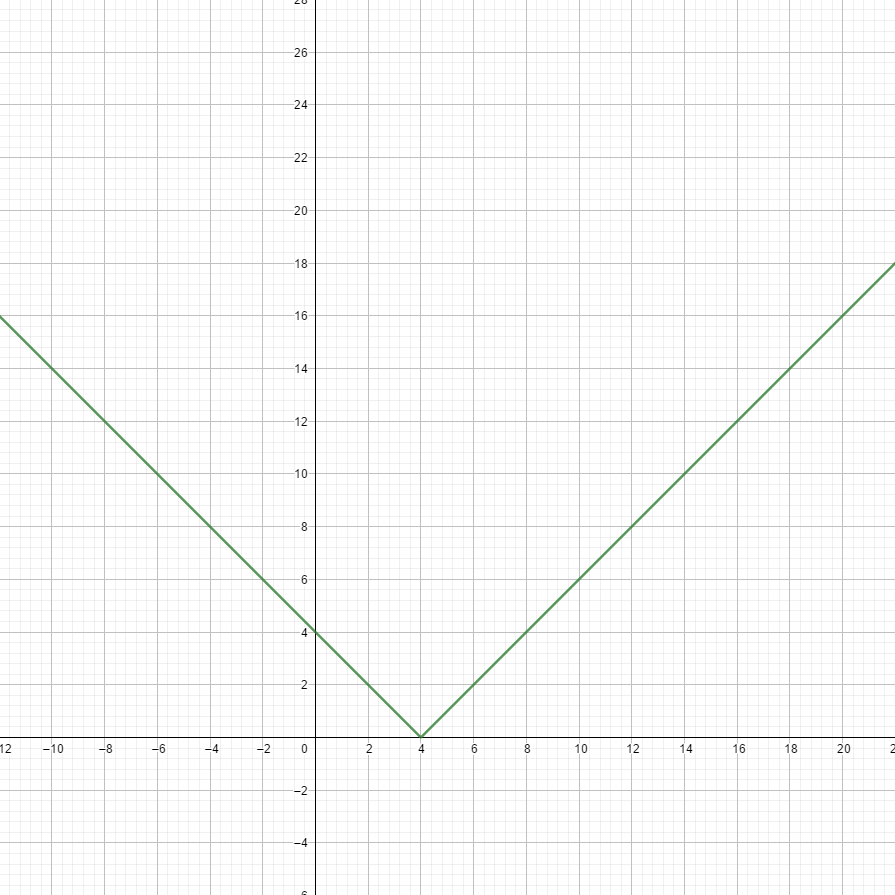
\includegraphics[width=\linewidth]{801a.png} %тут поменять имя пикчи
    \end{figure}
    \end{minipage}
\end{minipage}\\
$\spadesuit$}
{ВерныйОтвет}{Подсказка}
\end{problem}

\begin{problem}{Построение графика функции $y = f(x + a) + b$.}{8.3.3}{9I red есть ОДЗ}{*}
{Построить график функции $\displaystyle y(t) = 1 + \frac{3 \cdot ((t + 2)^{2} - 2t)}{\left(\sqrt{8 - t^{3}}\, \right)^{2}}$}
{НаписанноеРешение}
{ВерныйОтвет}{Подсказка}
\end{problem}

\begin{problem}{Построение графика функции $y = f(x + a) + b$.}{8.3.3}{9D}{(лёгкая)}
{Графически решить уравнение: \\
a) $|x - 3| + 1 = 2x$.
\\b) $|x + 3| - 1 = 2x$.}
{НаписанноеРешение}
{ВерныйОтвет}{Подсказка}
\end{problem}

\begin{problem}{Функция $y = ax^2 + bx + c$, её свойства и график.}{8.3.4}{7A}{(лёгкая)}
{Нарисовать график функции $y(x) = x^{2} - 5x + 4$.}
{НаписанноеРешение}
{ВерныйОтвет}{Подсказка}
\end{problem}

\begin{problem}{Функция $y = ax^2 + bx + c$, её свойства и график.}{8.3.4}{79I}{(лёгкая)}
{Для парабол $\displaystyle y_1(x) = x^{2} + 5x - 6$ и $\displaystyle y_2(x) = -x^{2} + 3x + 10$ соответствующие квадратные уравнения имеют равные дискриминанты.\\ Отобразить обе параболы на одном графике и найти у них равные элементы.}
{НаписанноеРешение}
{ВерныйОтвет}{Подсказка}
\end{problem}

\begin{problem}{Функция $y = ax^2 + bx + c$, её свойства и график.}{8.3.4}{79I}{(лёгкая)}
{Найти наибольшее значение функции $\,\displaystyle y = 3 - 10x - 25x^{2}$.}
{Перед нами уравнение параболы с ветвями, направленными вниз, поэтому наибольшее значение функции достигается в её вершине. Координата $x$ вершины параболы может быть найдена по формуле $x_{\text{в}} = -\frac{b}{2a}$, поэтому получаем $x_{\text{в}} = \frac{-(-10)}{2\cdot(-25)} = -\frac{1}{5} \;\Rightarrow\; y_{max} = y(-\frac{1}{5}) = 3 - 10\cdot(-\frac{1}{5})-25\cdot(-\frac{1}{5})^2 = 4$.}
{Наибольшее значение данной функции $y_{max} = 4$.}{График функции --- парабола.}
\end{problem}

\begin{problem}{Функция $y = ax^2 + bx + c$, её свойства и график.}{8.3.4}{79I}{(лёгкая)}
{Зависимость количества покупателей $N$ от цены товара имеет вид $N(p) = 6 - p$ ($p$~--- цена в тыс. руб.) Общая прибыль в этом случае зависит от цены и равна $r(p) = N(p) \cdot p$ тыс. руб. При какой цене прибыль максимальна?}
{$r(p) = N(p)\cdot p = (6-p)\cdot p = 6p-p^2$. Это уравнение параболы, старший коэффициент которой отрицателен, поэтому ветви параболы направлены вниз. Эта парабола достигает максимального значения в своей вершине $x_{\text{в}} = -\frac{6}{-2} = 3$. Прибыль будет равна $r_{max} = r(3) = 9$ тыс. руб.}
{При цене $p = 3$ прибыль максимальна и составляет 9 тыс. руб.}{График зависимости --- парабола.}
\end{problem}

\begin{problem}{Функция $y = ax^2 + bx + c$, её свойства и график.}{8.3.4}{79I}{(лёгкая)}
{Высота над землёй подброшенного вверх мяча меняется по закону $h(t) = 1{,}6 + 13t - 5t^{2}$, где $t$~--- время в секундах, прошедшее с момента броска, а $h$~--- высота в метрах. Через сколько секунд после момента броска мяч будет находиться на максимальной высоте? Чему равна эта высота?}
{Высота мяча над землёй $h(t)$ описывается параболой с отрицательным старшим коэффициентом $a = -5$. Значит, ветви этой параболы направлены вниз, и максимальная высота будет достигнута ровно в один определённый момент~--- когда мяч окажется в вершине этой параболы.\smallskip\\
$x$-координата вершины параболы $ax^2 + bx + c$ равна $x_{\text{в}} = -\frac{b}{2a}$, что в нашем случае даёт $-\frac{13}{2 \cdot (-5)} = 1{,}3$.\\ Значит, на максимальной высоте мяч окажется через $1{,}3$ секунды.\smallskip\\
$y$-координата вершины параболы $ax^2 + bx + c$ равна $y_{\text{в}} = -\frac{D}{4a}$, что в нашем случае равно $-\frac{13^2 - 4 \cdot (-5) \cdot 1{,}6}{4 \cdot (-5)} = \frac{169 + 32}{20} = 10{,}05$.\\ Поэтому максимальная высота, на которой окажется мяч, равна $10{,}05$ м.}
{Через $1{,}3$ с после момента броска мяч окажется на максимальной высоте, равной $10{,}05$ м.}{Подсказка}
\end{problem}

\begin{problem}{Функция $y = ax^2 + bx + c$, её свойства и график.}{8.3.4}{79I}{(лёгкая)}
{При каких значениях параметров $a$, $b$, $c$ парабола $y = ax^{2} + bx + c$:\\
a) Имеет 2 корня? \hfill b) Имеет 1 корень? \hfill с) Не имеет корней?\\
d) Пересекает ось ординат в точке с отрицательной координатой $y$?\\
Положим, что параметры таковы, что парабола всё же имеет 2 различных корня. В каком случае:\\
e) Сумма этих двух корней положительна? \\ f) Произведение этих двух корней положительно?\\ g) Оба корня отрицательны?}
{НаписанноеРешение}
{ВерныйОтвет}{Подсказка}
\end{problem}

\begin{problem}{Функция $y = ax^2 + bx + c$, её свойства и график.}{8.3.4}{79I}{(лёгкая)}
{Дан квадратный трёхчлен $y = ax^{2} + bx + c$.\\ Чему равны его значения в точках $x = 0$; $\,x = 1$; $\,x = -1$?}
{НаписанноеРешение}
{ВерныйОтвет}{Подсказка}
\end{problem}

\begin{problem}{Функция $y = ax^2 + bx + c$, её свойства и график.}{8.3.4}{79I}{*}
{Известно, что квадратный трёхчлен $y = ax^{2} + bx + c$ не имеет корней и $\,a + b + c > 0$.\\ Найти знак коэффициента $c$.}
{Трёхчлен не имеет корней, значит его график не пересекает ось $x$. По условию $a+b+c = y(1) > 0 \;\Rightarrow\;$ график лежит выше оси абсцисс, то есть находится в верхней полуплоскости. Следовательно $c = y(0)$ также больше нуля. }
{Коэффициент $c$ положителен.}{$a + b + c = y(1)$.}
\end{problem}

\begin{problem}{Функция $y = ax^2 + bx + c$, её свойства и график.}{8.3.4}{79I red параметр}{(лёгкая)}
{При каких значениях $p$ и $q$ график функции $\,\displaystyle y = x^{2} + px + q$ проходит через точки $A(1; -4)$ и $B(-2; 5)$?}
{НаписанноеРешение}
{ВерныйОтвет}{Подсказка}
\end{problem}

\begin{problem}{Функция $y = ax^2 + bx + c$, её свойства и график.}{8.3.4}{79I red параметр}{(лёгкая)}
{При каких значениях $p$ вершины парабол $\,\displaystyle y = x^{2} - 10px - 3$ и $y = x^{2} + 2px - 5p$ расположены в одной полуплоскости относительно оси абсцисс?}
{НаписанноеРешение}
{ВерныйОтвет}{Подсказка}
\end{problem}

\begin{problem}{Функция $y = ax^2 + bx + c$, её свойства и график.}{8.3.4}{9I \textcolor{olive}{\textbf{$\spadesuit$}}}{(лёгкая)}
{\vspace{-6mm}\\\begin{minipage}{\linewidth}
    \begin{minipage}{0.5\linewidth}

    Пользуясь графиком функции $y = ax^{2} + bx + c$, изображённым на рисунке, определить знаки чисел $a$, $b$, $c$, и дискриминанта $D$ квадратного трёхчлена $ax^{2} + bx + c$. Ответ объяснить.

    \end{minipage}
    \hspace{0.05\linewidth}
    \begin{minipage}{0.44\linewidth}
        \begin{figure}[H]
        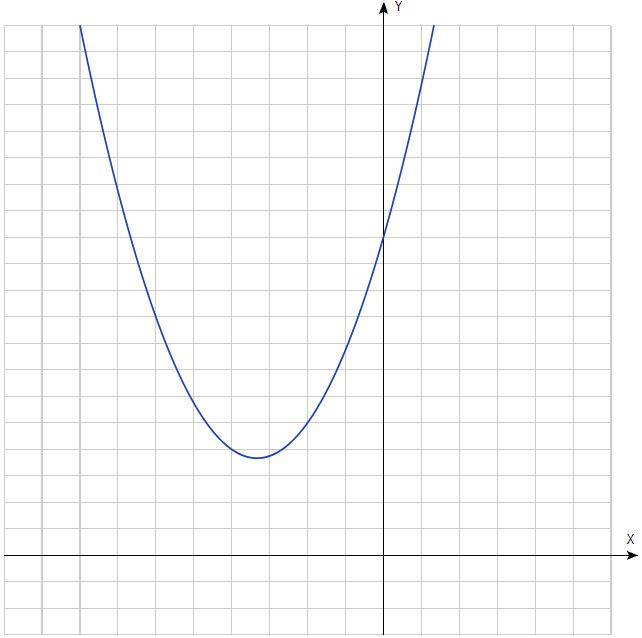
\includegraphics[width=\linewidth]{9I-3}
        \end{figure}
    \end{minipage}
\end{minipage}}
{Как видно из рисунка, ветви параболы направлены вверх.\\ Значит, старший коэффициент параболы, $a$, положителен.\smallskip\\ Свободный член параболы равен её значению в нуле: $y(0) = c$. Как мы можем видеть из рисунка, это значение также положительно.\smallskip\\ Дискриминант указывает на количество корней. В данном случае уравнение $y = 0$ корней не имеет (парабола не пересекается с осью абсцисс), поэтому $D < 0$.\smallskip\\ Оставшийся коэффициент $b$ определяет сдвиг параболы по горизонтали: поскольку $x_{\text{в}} = -\frac{b}{2a}$, и из рисунка видно, что вершина параболы имеет отрицательную координату, это означает, что $b > 0$. Итого, $a > 0$, $\,b > 0$, $\,c > 0$, $\,D < 0$.}
{$a$, $b$, $c$ --- положительны, $D$ отрицателен. Смотри рассуждения выше.}{Для данной параболы нужно определить направление ветвей, координату вершины, значение параболы в нуле, и количество корней.}
\end{problem}

\begin{problem}{Функция $y = ax^2 + bx + c$, её свойства и график.}{8.3.4}{9I red параметр}{(лёгкая)}
{Задать формулой квадратичную функцию, график которой проходит через точки $A = (-3; 2)$, $B = (1; -5)$, $C = (2; 7)$.}
{НаписанноеРешение}
{ВерныйОтвет}{Подсказка}
\end{problem}

\begin{problem}{Функция $y = ax^2 + bx + c$, её свойства и график.}{8.3.4}{9D}{(лёгкая)}
{Для функции $\displaystyle y(x) = \frac{x^{2} + 8x - 9}{3}$ найти:
\\a) Точку $A$ пересечения функции с осью ординат
\\b) Точку $B$ пересечения функции с осью абсцисс правее нуля
\\c) Точку $C$ пересечения функции с осью абсцисс левее нуля
\\d) Минимум функции
\\e) Расстояние между корнями, длину $BC$
\\f) Расстояние между точками $A$ и $B$, длину $AB$
\\g) Расстояние между точками $A$ и $C$, длину $AC$
\\h) Объяснение, почему $BC \cdot OA = AC \cdot AB$.}
{a) Чтобы найти точку пересечения графика функции с осью ординат, нужно найти значение этой функции в точке $x = 0$: $\;y(0) = \frac{0^2+8\cdot0-9}{3} = -3$.\\ Точка пересечения функции с осью ординат: $A = (0;-3)$.\smallskip\\
b)  Чтобы найти точку пересечения графика функции с осью абсцисс правее нуля, нужно приравнять функцию к 0, найти корни и выбрать из них положительный.\\
$y(x) = \frac{x^2+8x-9}{3} = 0 \;\Rightarrow\; x^2+8x-9 = 0.$ Решая, получаем два корня: $x = -9$ и $x = 1$. Точка пересечения функции с осью абсцисс правее нуля: $B = (1;0)$.\smallskip\\
c) В пункте b) мы нашли корни уравнения $y(x) = 0$, из которых теперь нужно выбрать отрицательное значение $x = -9$. Точка пересечения функции с осью абсцисс левее нуля: $C = (-9; 0)$.\smallskip\\
d) График нашей функции представляет собой параболу с ветвями вверх, поэтому минимум функции находится в вершине параболы. $x_{\text{в}} = \frac{-\frac83}{\frac23} = -4$.\\ Найдем значение функции в этой точке:
$\:y(-4) = \frac{(-4)^2+8(-4)-9}{3} = -\frac{25}{3} = -8\frac13$.\smallskip\\
e) $BC = x_B - x_C = 1 - (-9) = 10$.\smallskip\\
f) Расстояние между любыми двумя точками $(x_1; y_1)$ и $(x_2; y_2)$ на плоскости\\ находится по теореме Пифагора: $d = \sqrt{(x_1 - x_2)^2 + (y_1-y_2)^2}$. В нашем случае:\\
$AB = \sqrt{(0-1)^2+(-3-0)^2} = \sqrt{10}$.\smallskip\\
g) Аналогично $AC = \sqrt{(0-(-9))^2+(-3-0)^2} = 3\sqrt{10}$.\smallskip\\
h) Нетрудно заметить, что в данном случае треугольник $ABC$ --- прямоугольный (так как по обратной теореме Пифагора $BC^2 = 10^2 = 100 = 10 + 90 = AB^2 + AC^2$). Поэтому написанное --- подсчёт удвоенной площади треугольника $ABC$ двумя способами, так как для прямоугольного треугольника с гипотенузой $a$ и высотой $h$, проведённой к ней, $2S = a\cdot h = b \cdot c$.}
{Смотри рассуждения выше.}{Крайне полезно нарисовать график функции $y(x)$.\\ Для последнего пункта следует внимательно посмотреть на треугольник $ABC$.}
\end{problem}

\begin{problem}{Графическое решение уравнений-2.}{8.3.5}{7A}{(лёгкая)}
{Высота над землёй подброшенного вверх мяча меняется по закону $h(t) = 1 + 11t - 5t^{2}$, где $h$~--- высота в метрах, $t$~--- время в секундах, прошедшее с момента броска.\\ Сколько секунд мяч будет находиться на высоте не менее 3 метров?}
{Решим уравнение $h(t) = 3$:\\
$h(t) = 1 + 11t - 5t^2 = 3 \;\Rightarrow 5t^2 - 11t + 2 = 0$. Решаем уравнение, получаем два корня: $t = 2$ и $t = \frac{1}{5}$. Проанализируем полученный результат: поскольку по условию задачи мяч брошен снизу вверх, это означает, что в момент времени $t = 0{,}2$ секунды мяч находился на высоте 3 метра, двигаясь снизу вверх, а в момент времени $t = 2$ секунды мяч находился на этой высоте, двигаясь сверху вниз. Поэтому он находился на высоте не менее трех метров $2 - 0,2 = 1{,}8$ секунды.}
{Мяч находился на высоте не менее 3 метров всего $1{,}8$ секунды.}{Решить уравнение $h(t) = 3$.}
\end{problem}

\begin{problem}{Графическое решение уравнений-2.}{8.3.5}{7A}{(лёгкая)}
{Школьник в спортивном зале сильно пнул футбольный мяч вверх, в результате чего высота мяча над землёй до удара о стену меняется по закону $h(t) = -5t^{2} + 11t + 1$, где $t$ измеряется в секундах, а $h$~--- в метрах. Известно, что высота потолков в этом зале равна 7 метрам. Ударится ли мяч о потолок?}
{Чтобы узнать ударится ли мяч о потолок, нужно узнать, имеет ли вещественные корни уравнение $h(t) = 7$.\\
$h(t) = -5t^2+11t+1 = 7 \;\Rightarrow\; 5t^2-11t+6 = 0$. Дискриминант равен $121-120 = 1$, из этого следует, что уравнение имеет вещественные корни, а следовательно, мяч ударится о потолок.}
{Да, мяч ударится о потолок.}{Решить уравнение $h(t) = 7$.}
\end{problem}

\begin{problem}{Графическое решение уравнений-2.}{8.3.5}{7A red уравнения с модулем}{(лёгкая)}
{Построить график функции $y = |x + 1| - |x - 1| - x$ и найти все значения $k$, при которых прямая $y = kx$ имеет с графиком данной функции ровно одну общую точку.}
{НаписанноеРешение}
{ВерныйОтвет}{Подсказка}
\end{problem}

\begin{problem}{Графическое решение уравнений-2.}{8.3.5}{79I}{(лёгкая)}
{Зависимость объёма спроса $q$ на продукцию предприятия от цены $p$ (тыс. руб.) задаётся формулой $q = 160 - 10p$.\\ Выручка предприятия за месяц $r$ (тыс. руб.) вычисляется по формуле $r = q \cdot p$.\\ Определить наибольшую цену $p$, при которой выручка составит не менее 600 тыс. руб.}
{НаписанноеРешение}
{ВерныйОтвет}{Подсказка}
\end{problem}

\begin{problem}{Графическое решение уравнений-2.}{8.3.5}{79I \textcolor{red}{\textbf{$\spadesuit$}} или номер на замену, или тут надо свап, или сделать поучительным примером}{*}
{Решить уравнение: $\displaystyle x^{2} - |x| - 30 = 0$.}
{Проведём замену $|x| = t$ и решим квадратное уравнение:\\
$t^2 - t - 30 = 0 \;\Rightarrow\; t = 6$ или $t = -5$. Сделаем обратную замену:\\
1) $t = |x| =  6 \Rightarrow x = 6$ или $x = -6$.\\
2) $t = |x| = -5 \Rightarrow$ корней нет.} 
{Уравнение имеет два корня: $x = \pm 6$.}{Сделай замену $|x| = t$.}
\end{problem}

\begin{problem}{Графическое решение уравнений-2.}{8.3.5}{79I}{(лёгкая)}
{Найти наименьшее значение функции $y(x) = 4x^{2} - 16x + 19$.}
{График данной функции --- парабола с ветвями вверх, поэтому минимум функции достигается в её вершине. Координата вершины $x_{\text{в}} = \frac{-(-16)}{2\cdot4} = 2$.\\ Подставляем это значение в нашу функцию: $\,y(2) = 16 - 32 + 19 = 3$.}
{Наименьшее значение функции $y = 3$.}{Наименьшее значение функции достигается в вершине параболы.}
\end{problem}

\begin{problem}{Графическое решение уравнений-2.}{8.3.5}{79I}{(лёгкая)}
{Найти наибольшее значение функции $y(x) = 1 + 18t - 9t^{2}$.}
{Перед нами уравнение параболы с ветвями вниз, поэтому максимум функции будет в ее вершине. $x_{\text{в}} = \frac{-18}{-18} = 1 \;\Rightarrow\; y_{max} = y(1) = 1+18-9 = 10$.}
{Наибольшее значение функции  равно 10.}{Найди вершину параболы.}
\end{problem}

\begin{problem}{Графическое решение уравнений-2.}{8.3.5}{79I red параметр}{(лёгкая)}
{Найти все значения параметра $k$, при которых парабола $y = 12 - x^{2}$ и прямая $y = kx$ имеют ровно одну общую точку (прямая касается параболы)}
{Если прямая и парабола пересекаются в некоторой точке $(x_0; y_0)$, то для этой точки будут выполнены сразу оба уравнения. Поэтому задача сводится к нахождению таких $k$, что уравнение $12 - x^2 = kx$ имеет одно решение.\\ Перенесем все в одну часть, получим: $x^2 + kx - 12 = 0$. Дискриминант данного квадратного уравнения $D = k^2 + 48$ всегда больше нуля, поэтому для любых $k$ корней будет два, а значит прямая $kx$ будет пересекать параболу в двух точках.}
{Таких значений $k$ нет.}{Приравнять две функции и найти дискриминант.}
\end{problem}

\begin{problem}{Графическое решение уравнений-2.}{8.3.5}{79I}{(лёгкая)}
{При каком значении параметра $c$ наименьшее значение функции $\,\displaystyle y = 0{,}5x^{2} + 4x + c$ будет равно $-2$?}
{График данной функции --- парабола с ветвями вверх, поэтому минимум у функции будет в её вершине: $x_{\text{в}} = \frac{-4}{2\cdot0{,}5} = -4$.\\ Подставляем это значение в нашу функцию: $y(-4) = 0{,}5\cdot(-4)^2 + 4\cdot(-4) + c = -8 + c$. По условию это должно равняться $-2$, а значит $c = -2 + 8 = 6$.}
{Наименьшее значение функции равно $-2$ при $c = 6$.}{Наименьшее значение у параболы будет в её вершине.}
\end{problem}

\begin{problem}{Графическое решение уравнений-2.}{8.3.5}{9I red иррац урие}{(лёгкая)}
{Решить иррациональное уравнение $\sqrt{x + 8} + 1 = \sqrt{7x + 9}$.}
{НаписанноеРешение}
{ВерныйОтвет}{Подсказка}
\end{problem}

\begin{problem}{Графическое решение уравнений-2.}{8.3.5}{X red это параметр}{(лёгкая)}
{Есть две линии (дороги), $A$ и $B$, задаваемые уравнениями $y = cx^{2} - dx + 3$ и $y = dx^{2} - cx - 3$, соответственно. Известно, что эти две дороги пересекаются в точке с координатами $(-2; 3)$. Найти $c$ и $d$.\\ Выяснить, есть ли другие пересечения, и если есть, найти их координаты.}
{Раз мы точно знаем, что функции $y_1 = cx^{2} - dx + 3$ и $y_2 = dx^{2} - cx - 3$ пересекаются в точке $(-2; 3)$, выясним, какое уравнение мы из этого получаем.\smallskip\\ Во-первых, $y_1(-2) = 3 \;\Rightarrow\; c \cdot (-2)^2 - d \cdot (-2) + 3 = 3 \;\Rightarrow\; 4c + 2d = 0 \;\Rightarrow\; 2c + d = 0$.\\
Во-вторых, $y_2(-2) = 3 \;\Rightarrow\; d \cdot (-2)^2 - c \cdot (-2) - 3 = 3 \;\Rightarrow\; 4d + 2c = 6 \;\Rightarrow\; 2d + c = 3$.\\
В итоге получилась система линейных уравнений с двумя неизвестными:\\ $\left\{
\begin{aligned}
2c + d &= 0 \\
2d + c &= 3
\end{aligned}\right. \;\Rightarrow\; \left\{
\begin{aligned}
c &= -1 \\
d &= 2.
\end{aligned}\right.
\quad$ Итак, $c$ и $d$ успешно найдены.\smallskip\\ Проверим, есть ли другие пересечения: $y_1(x) = -x^2 - 2x + 3$, $y_2(x) = 2x^2 + x - 3$.\smallskip\\
Если пересечение есть, в нём $y_1(x) = y_2(x) \Rightarrow -x^2 - 2x + 3 = 2x^2 + x - 3 \Rightarrow 3x^2 + 3x - 6 = 0 \;\Rightarrow\; x^2 + x - 2 = 0 \;\Rightarrow\; (x - 1)(x + 2) = 0 \;\Rightarrow\; x = -2;\; x = 1$.\\ То есть пересечений два, и для второго пересечения $x = 1$,\; $y = -1 - 2 + 3 = 0$.}
{$c = -1$, $d = 2.$ Есть ещё одно пересечение, и оно происходит в точке $(1; 0)$.

}{Подсказка}
\end{problem}

\begin{problem}{Графическое решение уравнений-2.}{8.3.5}{X \textcolor{red}{\textbf{$\spadesuit$}} перенести в |f|}{*}
{Функция $\gamma(x)$ равна абсолютному значению функции $g(x) = 3x^{2} - x - 6$.
\\a) Сколько корней имеет уравнение $\gamma(x) = 4$? Найти сумму всех корней.
\\b) Аналогичный вопрос для уравнения $\gamma(x) = 2$. Найти сумму всех корней.}
{НаписанноеРешение}
{ВерныйОтвет}{Подсказка}
\end{problem}

\begin{problem}{Дробно-линейная функция.}{8.3.6}{79I}{(лёгкая)}
{Нарисовать график функции $\displaystyle y = \frac{x - 1}{5 - 2x}$, найти её асимптоты и растяжение по сравнению с обычной гиперболой $y = \frac{1}{x}$.}
{НаписанноеРешение}
{ВерныйОтвет}{Подсказка}
\end{problem}

\begin{problem}{Дробно-линейная функция.}{8.3.6}{79I red многопунктовая}{(лёгкая)}
{Изобразить графики гипербол, найти асимптоты и точки пересечения осей (при наличии)
\\a) $\displaystyle y = -1 + \frac{3}{x - 1}$
\hfill b) $\displaystyle y = \frac{-x + 2}{3x - 4}$
\hfill c) $\displaystyle x = 3 - \frac{2}{y + 1}$}
{НаписанноеРешение}
{ВерныйОтвет}{Подсказка}
\end{problem}

\begin{problem}{Дробно-линейная функция.}{8.3.6}{9D}{(лёгкая)}
{Построить график уравнения $xy = 3$.}
{НаписанноеРешение}
{ВерныйОтвет}{Подсказка}
\end{problem}

\begin{problem}{Дробно-линейная функция.}{8.3.6}{9D}{(лёгкая)}
{Построить график уравнения $xy + x = -5$.}
{НаписанноеРешение}
{ВерныйОтвет}{Подсказка}
\end{problem}

\begin{problem}{Дробно-линейная функция.}{8.3.6}{9D}{(лёгкая)}
{Построить график уравнения $(xy - 1)(y - 3) = 0$.}
{НаписанноеРешение}
{ВерныйОтвет}{Подсказка}
\end{problem}

\begin{problem}{Дробно-линейная функция.}{8.3.6}{9D}{(лёгкая)}
{Построить график уравнения $(xy - x + 5)(xy + y - 4) = 0$.}
{НаписанноеРешение}
{ВерныйОтвет}{Подсказка}
\end{problem}

\begin{problem}{Дробно-линейная функция.}{8.3.6}{9D}{(лёгкая)}
{Для гиперболы $\displaystyle y = a \cdot \frac{x - b}{x - c}$ найти асимптоты и центр.}
{НаписанноеРешение}
{ВерныйОтвет}{Подсказка}
\end{problem}

\begin{problem}{Дробно-линейная функция.}{8.3.6}{X}{(лёгкая)}
{Дана функция $\displaystyle y = f(x) = \frac{a}{x + b} + c$.\\ Нарисовать её график при $a = 2$, $b = -1$, $c = 3$. Что можно сказать о $a$, $b$, $c$, если рассуждать о растяжении и параллельных переносах?}
{НаписанноеРешение}
{ВерныйОтвет}{Подсказка}
\end{problem}

\begin{problem}{Построение графиков функций y = -f(x), y = f(-x), y = |f(x)|, и y = f(|x|).}{8.3.7}{7A}{(лёгкая)}
{Решить уравнение $\left|\vphantom{\frac{1}{1}}|3x - 9| - 2\right| = x - 1$ графически.}
{НаписанноеРешение}
{ВерныйОтвет}{Подсказка}
\end{problem}

\begin{problem}{Построение графиков функций y = -f(x), y = f(-x), y = |f(x)|, и y = f(|x|).}{8.3.7}{7A}{(лёгкая)}
{Решить уравнение $\left|\left|\frac{x - 5}{2}\right| - 1\right| = \left|\left|6 - 2x\right| - 5\right|$ графически.}
{НаписанноеРешение}
{ВерныйОтвет}{Подсказка}
\end{problem}

\begin{problem}{Построение графиков функций y = -f(x), y = f(-x), y = |f(x)|, и y = f(|x|).}{8.3.7}{7A}{(лёгкая)}
{Решить уравнение $\left|\frac{1}{4}(2x - 5)^{2} - \frac{5}{4}\right| = 1$, нарисовав график.}
{НаписанноеРешение}
{ВерныйОтвет}{Подсказка}
\end{problem}

\begin{problem}{Построение графиков функций y = -f(x), y = f(-x), y = |f(x)|, и y = f(|x|).}{8.3.7}{7A}{*}
{При каком $c$ уравнение $\left|(2x - 5)^{2} - 5\right| = c$ имеет 3 корня?}
{НаписанноеРешение}
{ВерныйОтвет}{Подсказка}
\end{problem}

\begin{problem}{Построение графиков функций y = -f(x), y = f(-x), y = |f(x)|, и y = f(|x|).}{8.3.7}{79I}{(лёгкая)}
{Построить график функции $y = |x^{2} + 2x - 8|$.}
{НаписанноеРешение}
{ВерныйОтвет}{Подсказка}
\end{problem}

\begin{problem}{Построение графиков функций y = -f(x), y = f(-x), y = |f(x)|, и y = f(|x|).}{8.3.7}{79I}{(лёгкая)}
{Построить график функции $y = x^{2} - 6|x| + 5$.}
{НаписанноеРешение}
{ВерныйОтвет}{Подсказка}
\end{problem}

\begin{problem}{Построение графиков функций y = -f(x), y = f(-x), y = |f(x)|, и y = f(|x|).}{8.3.7}{9I}{(лёгкая)}
{Решить уравнение $|x^{2} - 9| = 9 - x^{2}$ графически.}
{НаписанноеРешение}
{ВерныйОтвет}{Подсказка}
\end{problem}

\begin{problem}{Построение графиков функций y = -f(x), y = f(-x), y = |f(x)|, и y = f(|x|).}{8.3.7}{9D}{*}
{Нарисовать график функции $\displaystyle y(x) = \frac{x^{2}}{x^{2} - 4}$.}
{НаписанноеРешение}
{ВерныйОтвет}{Подсказка}
\end{problem}

\begin{problem}{Построение графиков функций y = -f(x), y = f(-x), y = |f(x)|, и y = f(|x|).}{8.3.7}{9D}{(лёгкая)}
{a) Построить график функции $y = x^{2} - 4x + 3$.\\
b) Построить график функции $y = |x^{2} - 4x + 3|$.\\
c) Построить график функции $y = x^{2} - 4|x| + 3$.}
{НаписанноеРешение}
{ВерныйОтвет}{Подсказка}
\end{problem}

\begin{problem}{Построение графиков функций y = -f(x), y = f(-x), y = |f(x)|, и y = f(|x|).}{8.3.7}{9D}{(лёгкая)}
{Решить уравнение $\displaystyle \left|\frac{1}{x}\right| = \frac{x + 3}{4}$ графически.}
{НаписанноеРешение}
{ВерныйОтвет}{Подсказка}
\end{problem}

\begin{problem}{Построение графиков функций y = -f(x), y = f(-x), y = |f(x)|, и y = f(|x|).}{8.3.7}{9D}{(лёгкая)}
{Установить, не решая, число корней уравнения
\\a) $\displaystyle \left|99x + 101\right| = 55$.
\\b) $\displaystyle \left|99x - 1001\right| = 0$.
\\с) $\displaystyle \left|11x + 9\right| = -3$.}
{а) Выражение под модулем, $99x + 101$, соответствует линейной функции и может принимать любые значения. Так как под модулем для решения может быть как $55$, так и $-55$, то уравнение имеет два корня.\smallskip\\
b) Уравнение будет иметь корень, когда $99x - 1001 = 0$, то есть в единственном случае.\smallskip\\
с) Уравнение не будет иметь ни единого корня, потому что левая часть уравнения всегда неотрицательна, а правая --- всегда отрицательна.}
{a) 2; $\quad$ b) 1; $\quad$ c) 0.}{Что можно сказать о знаках модуля и выражения внутри него?}
\end{problem}

\begin{problem}{Построение графиков функций y = -f(x), y = f(-x), y = |f(x)|, и y = f(|x|).}{8.3.7}{9D}{*}
{Дана функция $f(x) = ||||||x^{2} - 1| - 1| - 1| - 1| - 1| - 1|$. Известно, что для некоторых значений $x$ эта функция равна 3. Сколько решений имеет уравнение $f(x) = 3$?}
{НаписанноеРешение}
{ВерныйОтвет}{Подсказка}
\end{problem}

\begin{problem}{Построение графиков функций y = -f(x), y = f(-x), y = |f(x)|, и y = f(|x|).}{8.3.7}{9D}{*}
{Нарисовать по точкам график функции $\displaystyle y = g(x) = x + \frac{1}{x}$.\\ Судя по графику, сколько точек имеет координату $y$, равную $-1$?}
{НаписанноеРешение}
{ВерныйОтвет}{Подсказка}
\end{problem}

\begin{problem}{Построение графиков функций y = -f(x), y = f(-x), y = |f(x)|, и y = f(|x|).}{8.3.7}{X}{(лёгкая)}
{Решить уравнение $|3x - 2| + x = 11$ графически.}
{НаписанноеРешение}
{ВерныйОтвет}{Подсказка}
\end{problem}

\begin{problem}{Построение графиков функций y = -f(x), y = f(-x), y = |f(x)|, и y = f(|x|).}{8.3.7}{X}{(лёгкая)}
{Решить уравнение $\displaystyle \left|1 - \frac{x + 2}{3}\right| = \frac{7}{3}$ графически.}
{НаписанноеРешение}
{ВерныйОтвет}{Подсказка}
\end{problem}

\end{document}